% Options for packages loaded elsewhere
% Options for packages loaded elsewhere
\PassOptionsToPackage{unicode}{hyperref}
\PassOptionsToPackage{hyphens}{url}
\PassOptionsToPackage{dvipsnames,svgnames,x11names}{xcolor}
%
\documentclass[
  letterpaper,
  DIV=11,
  numbers=noendperiod]{scrartcl}
\usepackage{xcolor}
\usepackage{amsmath,amssymb}
\setcounter{secnumdepth}{-\maxdimen} % remove section numbering
\usepackage{iftex}
\ifPDFTeX
  \usepackage[T1]{fontenc}
  \usepackage[utf8]{inputenc}
  \usepackage{textcomp} % provide euro and other symbols
\else % if luatex or xetex
  \usepackage{unicode-math} % this also loads fontspec
  \defaultfontfeatures{Scale=MatchLowercase}
  \defaultfontfeatures[\rmfamily]{Ligatures=TeX,Scale=1}
\fi
\usepackage{lmodern}
\ifPDFTeX\else
  % xetex/luatex font selection
\fi
% Use upquote if available, for straight quotes in verbatim environments
\IfFileExists{upquote.sty}{\usepackage{upquote}}{}
\IfFileExists{microtype.sty}{% use microtype if available
  \usepackage[]{microtype}
  \UseMicrotypeSet[protrusion]{basicmath} % disable protrusion for tt fonts
}{}
\makeatletter
\@ifundefined{KOMAClassName}{% if non-KOMA class
  \IfFileExists{parskip.sty}{%
    \usepackage{parskip}
  }{% else
    \setlength{\parindent}{0pt}
    \setlength{\parskip}{6pt plus 2pt minus 1pt}}
}{% if KOMA class
  \KOMAoptions{parskip=half}}
\makeatother
% Make \paragraph and \subparagraph free-standing
\makeatletter
\ifx\paragraph\undefined\else
  \let\oldparagraph\paragraph
  \renewcommand{\paragraph}{
    \@ifstar
      \xxxParagraphStar
      \xxxParagraphNoStar
  }
  \newcommand{\xxxParagraphStar}[1]{\oldparagraph*{#1}\mbox{}}
  \newcommand{\xxxParagraphNoStar}[1]{\oldparagraph{#1}\mbox{}}
\fi
\ifx\subparagraph\undefined\else
  \let\oldsubparagraph\subparagraph
  \renewcommand{\subparagraph}{
    \@ifstar
      \xxxSubParagraphStar
      \xxxSubParagraphNoStar
  }
  \newcommand{\xxxSubParagraphStar}[1]{\oldsubparagraph*{#1}\mbox{}}
  \newcommand{\xxxSubParagraphNoStar}[1]{\oldsubparagraph{#1}\mbox{}}
\fi
\makeatother

\usepackage{color}
\usepackage{fancyvrb}
\newcommand{\VerbBar}{|}
\newcommand{\VERB}{\Verb[commandchars=\\\{\}]}
\DefineVerbatimEnvironment{Highlighting}{Verbatim}{commandchars=\\\{\}}
% Add ',fontsize=\small' for more characters per line
\usepackage{framed}
\definecolor{shadecolor}{RGB}{241,243,245}
\newenvironment{Shaded}{\begin{snugshade}}{\end{snugshade}}
\newcommand{\AlertTok}[1]{\textcolor[rgb]{0.68,0.00,0.00}{#1}}
\newcommand{\AnnotationTok}[1]{\textcolor[rgb]{0.37,0.37,0.37}{#1}}
\newcommand{\AttributeTok}[1]{\textcolor[rgb]{0.40,0.45,0.13}{#1}}
\newcommand{\BaseNTok}[1]{\textcolor[rgb]{0.68,0.00,0.00}{#1}}
\newcommand{\BuiltInTok}[1]{\textcolor[rgb]{0.00,0.23,0.31}{#1}}
\newcommand{\CharTok}[1]{\textcolor[rgb]{0.13,0.47,0.30}{#1}}
\newcommand{\CommentTok}[1]{\textcolor[rgb]{0.37,0.37,0.37}{#1}}
\newcommand{\CommentVarTok}[1]{\textcolor[rgb]{0.37,0.37,0.37}{\textit{#1}}}
\newcommand{\ConstantTok}[1]{\textcolor[rgb]{0.56,0.35,0.01}{#1}}
\newcommand{\ControlFlowTok}[1]{\textcolor[rgb]{0.00,0.23,0.31}{\textbf{#1}}}
\newcommand{\DataTypeTok}[1]{\textcolor[rgb]{0.68,0.00,0.00}{#1}}
\newcommand{\DecValTok}[1]{\textcolor[rgb]{0.68,0.00,0.00}{#1}}
\newcommand{\DocumentationTok}[1]{\textcolor[rgb]{0.37,0.37,0.37}{\textit{#1}}}
\newcommand{\ErrorTok}[1]{\textcolor[rgb]{0.68,0.00,0.00}{#1}}
\newcommand{\ExtensionTok}[1]{\textcolor[rgb]{0.00,0.23,0.31}{#1}}
\newcommand{\FloatTok}[1]{\textcolor[rgb]{0.68,0.00,0.00}{#1}}
\newcommand{\FunctionTok}[1]{\textcolor[rgb]{0.28,0.35,0.67}{#1}}
\newcommand{\ImportTok}[1]{\textcolor[rgb]{0.00,0.46,0.62}{#1}}
\newcommand{\InformationTok}[1]{\textcolor[rgb]{0.37,0.37,0.37}{#1}}
\newcommand{\KeywordTok}[1]{\textcolor[rgb]{0.00,0.23,0.31}{\textbf{#1}}}
\newcommand{\NormalTok}[1]{\textcolor[rgb]{0.00,0.23,0.31}{#1}}
\newcommand{\OperatorTok}[1]{\textcolor[rgb]{0.37,0.37,0.37}{#1}}
\newcommand{\OtherTok}[1]{\textcolor[rgb]{0.00,0.23,0.31}{#1}}
\newcommand{\PreprocessorTok}[1]{\textcolor[rgb]{0.68,0.00,0.00}{#1}}
\newcommand{\RegionMarkerTok}[1]{\textcolor[rgb]{0.00,0.23,0.31}{#1}}
\newcommand{\SpecialCharTok}[1]{\textcolor[rgb]{0.37,0.37,0.37}{#1}}
\newcommand{\SpecialStringTok}[1]{\textcolor[rgb]{0.13,0.47,0.30}{#1}}
\newcommand{\StringTok}[1]{\textcolor[rgb]{0.13,0.47,0.30}{#1}}
\newcommand{\VariableTok}[1]{\textcolor[rgb]{0.07,0.07,0.07}{#1}}
\newcommand{\VerbatimStringTok}[1]{\textcolor[rgb]{0.13,0.47,0.30}{#1}}
\newcommand{\WarningTok}[1]{\textcolor[rgb]{0.37,0.37,0.37}{\textit{#1}}}

\usepackage{longtable,booktabs,array}
\usepackage{calc} % for calculating minipage widths
% Correct order of tables after \paragraph or \subparagraph
\usepackage{etoolbox}
\makeatletter
\patchcmd\longtable{\par}{\if@noskipsec\mbox{}\fi\par}{}{}
\makeatother
% Allow footnotes in longtable head/foot
\IfFileExists{footnotehyper.sty}{\usepackage{footnotehyper}}{\usepackage{footnote}}
\makesavenoteenv{longtable}
\usepackage{graphicx}
\makeatletter
\newsavebox\pandoc@box
\newcommand*\pandocbounded[1]{% scales image to fit in text height/width
  \sbox\pandoc@box{#1}%
  \Gscale@div\@tempa{\textheight}{\dimexpr\ht\pandoc@box+\dp\pandoc@box\relax}%
  \Gscale@div\@tempb{\linewidth}{\wd\pandoc@box}%
  \ifdim\@tempb\p@<\@tempa\p@\let\@tempa\@tempb\fi% select the smaller of both
  \ifdim\@tempa\p@<\p@\scalebox{\@tempa}{\usebox\pandoc@box}%
  \else\usebox{\pandoc@box}%
  \fi%
}
% Set default figure placement to htbp
\def\fps@figure{htbp}
\makeatother





\setlength{\emergencystretch}{3em} % prevent overfull lines

\providecommand{\tightlist}{%
  \setlength{\itemsep}{0pt}\setlength{\parskip}{0pt}}



 


\KOMAoption{captions}{tableheading}
\makeatletter
\@ifpackageloaded{caption}{}{\usepackage{caption}}
\AtBeginDocument{%
\ifdefined\contentsname
  \renewcommand*\contentsname{Table of contents}
\else
  \newcommand\contentsname{Table of contents}
\fi
\ifdefined\listfigurename
  \renewcommand*\listfigurename{List of Figures}
\else
  \newcommand\listfigurename{List of Figures}
\fi
\ifdefined\listtablename
  \renewcommand*\listtablename{List of Tables}
\else
  \newcommand\listtablename{List of Tables}
\fi
\ifdefined\figurename
  \renewcommand*\figurename{Figure}
\else
  \newcommand\figurename{Figure}
\fi
\ifdefined\tablename
  \renewcommand*\tablename{Table}
\else
  \newcommand\tablename{Table}
\fi
}
\@ifpackageloaded{float}{}{\usepackage{float}}
\floatstyle{ruled}
\@ifundefined{c@chapter}{\newfloat{codelisting}{h}{lop}}{\newfloat{codelisting}{h}{lop}[chapter]}
\floatname{codelisting}{Listing}
\newcommand*\listoflistings{\listof{codelisting}{List of Listings}}
\makeatother
\makeatletter
\makeatother
\makeatletter
\@ifpackageloaded{caption}{}{\usepackage{caption}}
\@ifpackageloaded{subcaption}{}{\usepackage{subcaption}}
\makeatother
\usepackage{bookmark}
\IfFileExists{xurl.sty}{\usepackage{xurl}}{} % add URL line breaks if available
\urlstyle{same}
\hypersetup{
  pdftitle={Class 10: Structural Bioinformatics 1},
  pdfauthor={Raneem Kassar (PID: A17803411)},
  colorlinks=true,
  linkcolor={blue},
  filecolor={Maroon},
  citecolor={Blue},
  urlcolor={Blue},
  pdfcreator={LaTeX via pandoc}}


\title{Class 10: Structural Bioinformatics 1}
\author{Raneem Kassar (PID: A17803411)}
\date{}
\begin{document}
\maketitle


\subsection{Background}\label{background}

The main repository of high-resolution structural data on biomolecules
is called the \textbf{Protein Data Bank}(PDB).

\subsection{PDB Statistics}\label{pdb-statistics}

What in in the PDB in terms of molecule type and structure determination
method?

Read a CSV file of current PDB stats from
https://www.rcsb.org/stats/summary

\begin{Shaded}
\begin{Highlighting}[]
\NormalTok{pdb }\OtherTok{\textless{}{-}} \FunctionTok{read.csv}\NormalTok{(}\StringTok{"Data Export Summary.csv"}\NormalTok{)}
\NormalTok{pdb }
\end{Highlighting}
\end{Shaded}

\begin{verbatim}
           Molecular.Type   X.ray     EM    NMR Integrative Multiple.methods
1          Protein (only) 180,758 23,111 12,813         348              229
2 Protein/Oligosaccharide  10,488  3,741     34           8               11
3              Protein/NA   9,205  6,751    287          26                8
4     Nucleic acid (only)   3,154    250  1,578           3               15
5                   Other     178     27     35           4                0
6  Oligosaccharide (only)      11      0      6           0                1
  Neutron Other   Total
1      84    32 217,375
2       1     0  14,283
3       0     0  16,277
4       3     1   5,004
5       0     0     244
6       0     4      22
\end{verbatim}

\begin{Shaded}
\begin{Highlighting}[]
\NormalTok{pdb}\SpecialCharTok{$}\NormalTok{X.ray}
\end{Highlighting}
\end{Shaded}

\begin{verbatim}
[1] "180,758" "10,488"  "9,205"   "3,154"   "178"     "11"     
\end{verbatim}

This print out above is \texttt{pdb\$X.ray} is ``character'' not
``numeric''. Therefore I can't do math with it. We need to fix
this\ldots{}

Two functions that can help here are \texttt{sub()} and
\texttt{as.numeric()}

\begin{Shaded}
\begin{Highlighting}[]
\CommentTok{\# We want to get rid (or sub out) commas:}
\NormalTok{x }\OtherTok{\textless{}{-}}\NormalTok{ pdb}\SpecialCharTok{$}\NormalTok{X.ray}
\NormalTok{tmp }\OtherTok{\textless{}{-}} \FunctionTok{sub}\NormalTok{(}\StringTok{","}\NormalTok{, }\StringTok{""}\NormalTok{, x)}
\FunctionTok{sum}\NormalTok{( }\FunctionTok{as.numeric}\NormalTok{(tmp) )}
\end{Highlighting}
\end{Shaded}

\begin{verbatim}
[1] 203794
\end{verbatim}

We could make a function to do this:

\begin{Shaded}
\begin{Highlighting}[]
\NormalTok{rm.comma }\OtherTok{\textless{}{-}} \ControlFlowTok{function}\NormalTok{(x) \{}
\NormalTok{  tmp }\OtherTok{\textless{}{-}} \FunctionTok{sub}\NormalTok{(}\StringTok{","}\NormalTok{, }\StringTok{""}\NormalTok{, x)}
\FunctionTok{sum}\NormalTok{( }\FunctionTok{as.numeric}\NormalTok{(tmp) )}
\NormalTok{\}}
\end{Highlighting}
\end{Shaded}

\begin{quote}
Q1: What percentage of structures in the PDB are solved by X-Ray and
Electron Microscopy.
\end{quote}

\begin{Shaded}
\begin{Highlighting}[]
\NormalTok{n.tot  }\OtherTok{\textless{}{-}} \FunctionTok{rm.comma}\NormalTok{(pdb}\SpecialCharTok{$}\NormalTok{Total)}
\NormalTok{n.xray }\OtherTok{\textless{}{-}} \FunctionTok{rm.comma}\NormalTok{(pdb}\SpecialCharTok{$}\NormalTok{X.ray)}
\NormalTok{n.em   }\OtherTok{\textless{}{-}} \FunctionTok{rm.comma}\NormalTok{(pdb}\SpecialCharTok{$}\NormalTok{EM)}

\NormalTok{n.xray}\SpecialCharTok{/}\NormalTok{n.tot }\SpecialCharTok{*} \DecValTok{100}
\end{Highlighting}
\end{Shaded}

\begin{verbatim}
[1] 80.48577
\end{verbatim}

\begin{Shaded}
\begin{Highlighting}[]
\NormalTok{n.em}\SpecialCharTok{/}\NormalTok{n.tot }\SpecialCharTok{*} \DecValTok{100}
\end{Highlighting}
\end{Shaded}

\begin{verbatim}
[1] 13.38046
\end{verbatim}

We could also use a different import function \texttt{read\_csv()} for
this CSV that speaks American (i.e.~deals with commas in numbers in a
comma seperated value file).

\begin{Shaded}
\begin{Highlighting}[]
\FunctionTok{library}\NormalTok{(readr)}

\NormalTok{pdb }\OtherTok{\textless{}{-}} \FunctionTok{read\_csv}\NormalTok{(}\StringTok{"Data Export Summary.csv"}\NormalTok{)}
\end{Highlighting}
\end{Shaded}

\begin{verbatim}
Rows: 6 Columns: 9
-- Column specification --------------------------------------------------------
Delimiter: ","
chr (1): Molecular Type
dbl (4): Integrative, Multiple methods, Neutron, Other
num (4): X-ray, EM, NMR, Total

i Use `spec()` to retrieve the full column specification for this data.
i Specify the column types or set `show_col_types = FALSE` to quiet this message.
\end{verbatim}

\begin{Shaded}
\begin{Highlighting}[]
\NormalTok{n.tot }\OtherTok{\textless{}{-}}\NormalTok{ (pdb}\SpecialCharTok{$}\NormalTok{Total)}
\NormalTok{n.xray }\OtherTok{\textless{}{-}} \FunctionTok{sum}\NormalTok{(pdb}\SpecialCharTok{$}\StringTok{\textasciigrave{}}\AttributeTok{X{-}ray}\StringTok{\textasciigrave{}}\NormalTok{)}
\FunctionTok{sum}\NormalTok{(pdb}\SpecialCharTok{$}\StringTok{\textasciigrave{}}\AttributeTok{X{-}ray}\StringTok{\textasciigrave{}}\NormalTok{) }\SpecialCharTok{/}\NormalTok{ n.tot}
\end{Highlighting}
\end{Shaded}

\begin{verbatim}
[1]    0.9375227   14.2682910   12.5203662   40.7262190  835.2213115
[6] 9263.3636364
\end{verbatim}

\begin{Shaded}
\begin{Highlighting}[]
\NormalTok{n.xray }\SpecialCharTok{/}\NormalTok{ n.tot }\SpecialCharTok{*} \DecValTok{100}
\end{Highlighting}
\end{Shaded}

\begin{verbatim}
[1]     93.75227   1426.82910   1252.03662   4072.62190  83522.13115
[6] 926336.36364
\end{verbatim}

\begin{Shaded}
\begin{Highlighting}[]
\NormalTok{n.em }\SpecialCharTok{/}\NormalTok{ n.tot }\SpecialCharTok{*} \DecValTok{100}
\end{Highlighting}
\end{Shaded}

\begin{verbatim}
[1]     15.58597    237.20507    208.14646    677.05835  13885.24590
[6] 154000.00000
\end{verbatim}

\begin{Shaded}
\begin{Highlighting}[]
\NormalTok{pdb}\SpecialCharTok{$}\NormalTok{Total[}\DecValTok{1}\NormalTok{]}
\end{Highlighting}
\end{Shaded}

\begin{verbatim}
[1] 217375
\end{verbatim}

\begin{quote}
Q. How many protein structures are in this dataset?
\end{quote}

\begin{Shaded}
\begin{Highlighting}[]
\DecValTok{217375}\SpecialCharTok{/}\DecValTok{2025556314} \SpecialCharTok{*} \DecValTok{100}
\end{Highlighting}
\end{Shaded}

\begin{verbatim}
[1] 0.01073162
\end{verbatim}

\begin{quote}
Q2: What proportion of structures in the PDB are protein?
\end{quote}

\begin{Shaded}
\begin{Highlighting}[]
\FunctionTok{names}\NormalTok{(pdb)}
\end{Highlighting}
\end{Shaded}

\begin{verbatim}
[1] "Molecular Type"   "X-ray"            "EM"               "NMR"             
[5] "Integrative"      "Multiple methods" "Neutron"          "Other"           
[9] "Total"           
\end{verbatim}

\begin{Shaded}
\begin{Highlighting}[]
\FunctionTok{library}\NormalTok{(readr)}

\NormalTok{pdb\_stats }\OtherTok{\textless{}{-}} \FunctionTok{read\_csv}\NormalTok{(}\StringTok{"Data Export Summary.csv"}\NormalTok{)}
\end{Highlighting}
\end{Shaded}

\begin{verbatim}
Rows: 6 Columns: 9
-- Column specification --------------------------------------------------------
Delimiter: ","
chr (1): Molecular Type
dbl (4): Integrative, Multiple methods, Neutron, Other
num (4): X-ray, EM, NMR, Total

i Use `spec()` to retrieve the full column specification for this data.
i Specify the column types or set `show_col_types = FALSE` to quiet this message.
\end{verbatim}

\begin{Shaded}
\begin{Highlighting}[]
\NormalTok{protein\_rows }\OtherTok{\textless{}{-}} \FunctionTok{grepl}\NormalTok{(}\StringTok{"Protein"}\NormalTok{, pdb\_stats}\SpecialCharTok{$}\StringTok{\textasciigrave{}}\AttributeTok{Molecular Type}\StringTok{\textasciigrave{}}\NormalTok{)}

\NormalTok{protein\_total }\OtherTok{\textless{}{-}} \FunctionTok{sum}\NormalTok{(pdb\_stats}\SpecialCharTok{$}\NormalTok{Total[protein\_rows])}
\NormalTok{total\_structures }\OtherTok{\textless{}{-}} \FunctionTok{sum}\NormalTok{(pdb\_stats}\SpecialCharTok{$}\NormalTok{Total)}

\NormalTok{protein\_total }\SpecialCharTok{/}\NormalTok{ total\_structures}
\end{Highlighting}
\end{Shaded}

\begin{verbatim}
[1] 0.9791868
\end{verbatim}

\begin{Shaded}
\begin{Highlighting}[]
\NormalTok{protein\_total }\SpecialCharTok{/}\NormalTok{ total\_structures }\SpecialCharTok{*} \DecValTok{100}
\end{Highlighting}
\end{Shaded}

\begin{verbatim}
[1] 97.91868
\end{verbatim}

The proportion of structure in the PDB that are protein are 98\%.

\begin{quote}
\textbf{Key-point}: We have a very, very small structural coverage of
known proteins (\textasciitilde0.1\%). Most structures we know about
(\textasciitilde80\%) come from one method (X-ray crystalography).
\end{quote}

\subsection{Visualizing PDB data with
Mol-star}\label{visualizing-pdb-data-with-mol-star}

Main stand alone website with all features is at
https://molstar.org/viewer/

\begin{figure}[H]

{\centering \pandocbounded{\includegraphics[keepaspectratio]{1HSG.png}}

}

\caption{The HIV-protease enzyme is a homodimer with two chains}

\end{figure}%

\begin{figure}[H]

{\centering \pandocbounded{\includegraphics[keepaspectratio]{1HSG_surf.png}}

}

\caption{Surface display showing the binding cleft site foe the
inhibitor drug molecule}

\end{figure}%

\begin{figure}[H]

{\centering \pandocbounded{\includegraphics[keepaspectratio]{1HSG_Asp25.png}}

}

\caption{Spacefill display of catalytic ASP25 amino acids and binding
site water molecule}

\end{figure}%

\section{Getting started with the Bio3d
package}\label{getting-started-with-the-bio3d-package}

Bio3D is an R package from CRAN for structural bioinformatics

\begin{Shaded}
\begin{Highlighting}[]
\FunctionTok{library}\NormalTok{(bio3d)}

\NormalTok{pdb }\OtherTok{\textless{}{-}} \FunctionTok{read.pdb}\NormalTok{(}\StringTok{"1hsg"}\NormalTok{)}
\end{Highlighting}
\end{Shaded}

\begin{verbatim}
  Note: Accessing on-line PDB file
\end{verbatim}

\begin{Shaded}
\begin{Highlighting}[]
\NormalTok{pdb}
\end{Highlighting}
\end{Shaded}

\begin{verbatim}

 Call:  read.pdb(file = "1hsg")

   Total Models#: 1
     Total Atoms#: 1686,  XYZs#: 5058  Chains#: 2  (values: A B)

     Protein Atoms#: 1514  (residues/Calpha atoms#: 198)
     Nucleic acid Atoms#: 0  (residues/phosphate atoms#: 0)

     Non-protein/nucleic Atoms#: 172  (residues: 128)
     Non-protein/nucleic resid values: [ HOH (127), MK1 (1) ]

   Protein sequence:
      PQITLWQRPLVTIKIGGQLKEALLDTGADDTVLEEMSLPGRWKPKMIGGIGGFIKVRQYD
      QILIEICGHKAIGTVLVGPTPVNIIGRNLLTQIGCTLNFPQITLWQRPLVTIKIGGQLKE
      ALLDTGADDTVLEEMSLPGRWKPKMIGGIGGFIKVRQYDQILIEICGHKAIGTVLVGPTP
      VNIIGRNLLTQIGCTLNF

+ attr: atom, xyz, seqres, helix, sheet,
        calpha, remark, call
\end{verbatim}

\begin{Shaded}
\begin{Highlighting}[]
\FunctionTok{head}\NormalTok{(pdb}\SpecialCharTok{$}\NormalTok{atom, }\DecValTok{5}\NormalTok{)}
\end{Highlighting}
\end{Shaded}

\begin{verbatim}
  type eleno elety  alt resid chain resno insert      x      y     z o     b
1 ATOM     1     N <NA>   PRO     A     1   <NA> 29.361 39.686 5.862 1 38.10
2 ATOM     2    CA <NA>   PRO     A     1   <NA> 30.307 38.663 5.319 1 40.62
3 ATOM     3     C <NA>   PRO     A     1   <NA> 29.760 38.071 4.022 1 42.64
4 ATOM     4     O <NA>   PRO     A     1   <NA> 28.600 38.302 3.676 1 43.40
5 ATOM     5    CB <NA>   PRO     A     1   <NA> 30.508 37.541 6.342 1 37.87
  segid elesy charge
1  <NA>     N   <NA>
2  <NA>     C   <NA>
3  <NA>     C   <NA>
4  <NA>     O   <NA>
5  <NA>     C   <NA>
\end{verbatim}

There are lots of functions that can work with these \texttt{pdb}
objects

\begin{Shaded}
\begin{Highlighting}[]
\FunctionTok{head}\NormalTok{ ( }\FunctionTok{pdbseq}\NormalTok{( pdb) )}
\end{Highlighting}
\end{Shaded}

\begin{verbatim}
  1   2   3   4   5   6 
"P" "Q" "I" "T" "L" "W" 
\end{verbatim}

We can have a quick interactive view of any of these \texttt{pdb}
objects:

\begin{Shaded}
\begin{Highlighting}[]
\FunctionTok{library}\NormalTok{(bio3dview)}

\CommentTok{\#view.pdb(pdb)}
\end{Highlighting}
\end{Shaded}

Let's try a custom view

\begin{Shaded}
\begin{Highlighting}[]
\CommentTok{\#view.pdb(pdb, colorScheme="sse",}
\CommentTok{\#         backgroundColor="black")}
\end{Highlighting}
\end{Shaded}

\begin{quote}
Q. Create a custom view of HIV-Prhighlighting the active site ASP
(\texttt{resno=25}), the two chains (in your choice of colors) and the
ligand all on a custom color background?
\end{quote}

\begin{Shaded}
\begin{Highlighting}[]
\FunctionTok{library}\NormalTok{(NGLVieweR)}

\NormalTok{active.site }\OtherTok{\textless{}{-}} \FunctionTok{atom.select}\NormalTok{(pdb, }\AttributeTok{resno=}\DecValTok{25}\NormalTok{)}

\CommentTok{\#view.pdb(pdb, }
\CommentTok{\#         cols= c("red", "blue"),}
\CommentTok{\#         highlight = active.site, }
\CommentTok{\#         highlight.style = "spacefill",}
\CommentTok{\#         backgroundColor="pink") |\textgreater{}}
\CommentTok{\#  setRock()}
\end{Highlighting}
\end{Shaded}

\subsection{Predict the flexibility of a given
structure}\label{predict-the-flexibility-of-a-given-structure}

Let's do a Normal Mode Analysis (NMA) to predict the flexibility of a
give \texttt{pdb} object:

\begin{Shaded}
\begin{Highlighting}[]
\NormalTok{adk }\OtherTok{\textless{}{-}} \FunctionTok{read.pdb}\NormalTok{(}\StringTok{"6s36"}\NormalTok{)}
\end{Highlighting}
\end{Shaded}

\begin{verbatim}
  Note: Accessing on-line PDB file
   PDB has ALT records, taking A only, rm.alt=TRUE
\end{verbatim}

A quick structure summary

\begin{Shaded}
\begin{Highlighting}[]
\NormalTok{adk}
\end{Highlighting}
\end{Shaded}

\begin{verbatim}

 Call:  read.pdb(file = "6s36")

   Total Models#: 1
     Total Atoms#: 1898,  XYZs#: 5694  Chains#: 1  (values: A)

     Protein Atoms#: 1654  (residues/Calpha atoms#: 214)
     Nucleic acid Atoms#: 0  (residues/phosphate atoms#: 0)

     Non-protein/nucleic Atoms#: 244  (residues: 244)
     Non-protein/nucleic resid values: [ CL (3), HOH (238), MG (2), NA (1) ]

   Protein sequence:
      MRIILLGAPGAGKGTQAQFIMEKYGIPQISTGDMLRAAVKSGSELGKQAKDIMDAGKLVT
      DELVIALVKERIAQEDCRNGFLLDGFPRTIPQADAMKEAGINVDYVLEFDVPDELIVDKI
      VGRRVHAPSGRVYHVKFNPPKVEGKDDVTGEELTTRKDDQEETVRKRLVEYHQMTAPLIG
      YYSKEAEAGNTKYAKVDGTKPVAEVRADLEKILG

+ attr: atom, xyz, seqres, helix, sheet,
        calpha, remark, call
\end{verbatim}

\begin{Shaded}
\begin{Highlighting}[]
\NormalTok{m }\OtherTok{\textless{}{-}} \FunctionTok{nma}\NormalTok{( adk )}
\end{Highlighting}
\end{Shaded}

\begin{verbatim}
 Building Hessian...        Done in 0.009 seconds.
 Diagonalizing Hessian...   Done in 0.175 seconds.
\end{verbatim}

\begin{Shaded}
\begin{Highlighting}[]
\FunctionTok{plot}\NormalTok{(m)}
\end{Highlighting}
\end{Shaded}

\pandocbounded{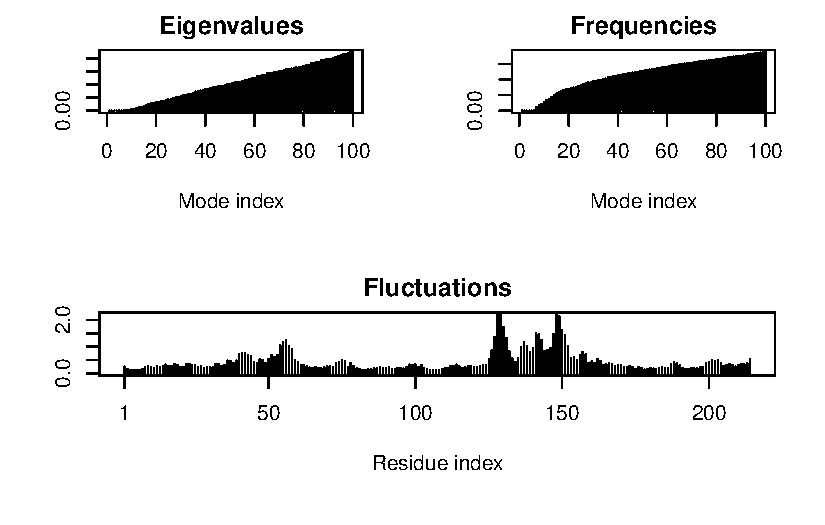
\includegraphics[keepaspectratio]{Class10_files/figure-pdf/unnamed-chunk-20-1.pdf}}

View the results with an interactive structure view:

\begin{Shaded}
\begin{Highlighting}[]
\CommentTok{\#view.nma(m)}
\end{Highlighting}
\end{Shaded}

Write out the results for viewing in Mol-star:

\begin{Shaded}
\begin{Highlighting}[]
\FunctionTok{mktrj}\NormalTok{(m, }\AttributeTok{file=}\StringTok{"nma.pdb"}\NormalTok{)}
\end{Highlighting}
\end{Shaded}

\begin{quote}
Q10. Which of the packages above is found only on BioConductor and not
CRAN?
\end{quote}

The package found only on BioConductor is ``msa.''

\begin{quote}
Q11. Which of the above packages is not found on BioConductor or CRAN?:
\end{quote}

The above packages that is not found on BioConductor or CRAN is
``bio3d\#view.''

\begin{quote}
Q12. True or False? Functions from the pak package can be used to
install packages from GitHub and BitBucket?
\end{quote}

True.

\subsection{Comparative analysis of the ADK
family}\label{comparative-analysis-of-the-adk-family}

Our first step is find a sequence for this family. We will use the
databse ID ``1ake\_A'' here:

\begin{Shaded}
\begin{Highlighting}[]
\NormalTok{id }\OtherTok{\textless{}{-}} \StringTok{"1ake\_A"}

\NormalTok{aa }\OtherTok{\textless{}{-}} \FunctionTok{get.seq}\NormalTok{(id)}
\end{Highlighting}
\end{Shaded}

\begin{verbatim}
Warning in get.seq(id): Removing existing file: seqs.fasta
\end{verbatim}

\begin{verbatim}
Fetching... Please wait. Done.
\end{verbatim}

\begin{Shaded}
\begin{Highlighting}[]
\NormalTok{aa}
\end{Highlighting}
\end{Shaded}

\begin{verbatim}
             1        .         .         .         .         .         60 
pdb|1AKE|A   MRIILLGAPGAGKGTQAQFIMEKYGIPQISTGDMLRAAVKSGSELGKQAKDIMDAGKLVT
             1        .         .         .         .         .         60 

            61        .         .         .         .         .         120 
pdb|1AKE|A   DELVIALVKERIAQEDCRNGFLLDGFPRTIPQADAMKEAGINVDYVLEFDVPDELIVDRI
            61        .         .         .         .         .         120 

           121        .         .         .         .         .         180 
pdb|1AKE|A   VGRRVHAPSGRVYHVKFNPPKVEGKDDVTGEELTTRKDDQEETVRKRLVEYHQMTAPLIG
           121        .         .         .         .         .         180 

           181        .         .         .   214 
pdb|1AKE|A   YYSKEAEAGNTKYAKVDGTKPVAEVRADLEKILG
           181        .         .         .   214 

Call:
  read.fasta(file = outfile)

Class:
  fasta

Alignment dimensions:
  1 sequence rows; 214 position columns (214 non-gap, 0 gap) 

+ attr: id, ali, call
\end{verbatim}

\begin{quote}
Q13. How many amino acids are in this sequence, i.e.~how long is this
sequence?
\end{quote}

There are 214 amino acids in this sequence.

Search for related sequences in the database

\begin{Shaded}
\begin{Highlighting}[]
\CommentTok{\#blast \textless{}{-} blast.pdb(aa)}
\end{Highlighting}
\end{Shaded}

\begin{Shaded}
\begin{Highlighting}[]
\CommentTok{\#head(blast$hit.tbl)}
\end{Highlighting}
\end{Shaded}

\begin{Shaded}
\begin{Highlighting}[]
\CommentTok{\#hits \textless{}{-} plot(blast)}
\end{Highlighting}
\end{Shaded}

\begin{Shaded}
\begin{Highlighting}[]
\NormalTok{hits }\OtherTok{\textless{}{-}} \ConstantTok{NULL}
\NormalTok{hits}\SpecialCharTok{$}\NormalTok{pdb.id }\OtherTok{\textless{}{-}} \FunctionTok{c}\NormalTok{(}\StringTok{\textquotesingle{}1AKE\_A\textquotesingle{}}\NormalTok{,}\StringTok{\textquotesingle{}6S36\_A\textquotesingle{}}\NormalTok{,}\StringTok{\textquotesingle{}6RZE\_A\textquotesingle{}}\NormalTok{,}\StringTok{\textquotesingle{}3HPR\_A\textquotesingle{}}\NormalTok{,}\StringTok{\textquotesingle{}1E4V\_A\textquotesingle{}}\NormalTok{,}\StringTok{\textquotesingle{}5EJE\_A\textquotesingle{}}\NormalTok{,}\StringTok{\textquotesingle{}1E4Y\_A\textquotesingle{}}\NormalTok{,}\StringTok{\textquotesingle{}3X2S\_A\textquotesingle{}}\NormalTok{,}\StringTok{\textquotesingle{}6HAP\_A\textquotesingle{}}\NormalTok{,}\StringTok{\textquotesingle{}6HAM\_A\textquotesingle{}}\NormalTok{,}\StringTok{\textquotesingle{}4K46\_A\textquotesingle{}}\NormalTok{,}\StringTok{\textquotesingle{}3GMT\_A\textquotesingle{}}\NormalTok{,}\StringTok{\textquotesingle{}4PZL\_A\textquotesingle{}}\NormalTok{)}
\end{Highlighting}
\end{Shaded}

\begin{Shaded}
\begin{Highlighting}[]
\NormalTok{hits}\SpecialCharTok{$}\NormalTok{pdb.id}
\end{Highlighting}
\end{Shaded}

\begin{verbatim}
 [1] "1AKE_A" "6S36_A" "6RZE_A" "3HPR_A" "1E4V_A" "5EJE_A" "1E4Y_A" "3X2S_A"
 [9] "6HAP_A" "6HAM_A" "4K46_A" "3GMT_A" "4PZL_A"
\end{verbatim}

\begin{Shaded}
\begin{Highlighting}[]
\NormalTok{files }\OtherTok{\textless{}{-}}\FunctionTok{get.pdb}\NormalTok{(hits}\SpecialCharTok{$}\NormalTok{pdb.id, }\AttributeTok{path=}\StringTok{"pdbs"}\NormalTok{, }\AttributeTok{split=}\ConstantTok{TRUE}\NormalTok{, }\AttributeTok{gzip=}\ConstantTok{TRUE}\NormalTok{)}
\end{Highlighting}
\end{Shaded}

\begin{verbatim}
Warning in get.pdb(hits$pdb.id, path = "pdbs", split = TRUE, gzip = TRUE):
pdbs/1AKE.pdb.gz exists. Skipping download
\end{verbatim}

\begin{verbatim}
Warning in get.pdb(hits$pdb.id, path = "pdbs", split = TRUE, gzip = TRUE):
pdbs/6S36.pdb.gz exists. Skipping download
\end{verbatim}

\begin{verbatim}
Warning in get.pdb(hits$pdb.id, path = "pdbs", split = TRUE, gzip = TRUE):
pdbs/6RZE.pdb.gz exists. Skipping download
\end{verbatim}

\begin{verbatim}
Warning in get.pdb(hits$pdb.id, path = "pdbs", split = TRUE, gzip = TRUE):
pdbs/3HPR.pdb.gz exists. Skipping download
\end{verbatim}

\begin{verbatim}
Warning in get.pdb(hits$pdb.id, path = "pdbs", split = TRUE, gzip = TRUE):
pdbs/1E4V.pdb.gz exists. Skipping download
\end{verbatim}

\begin{verbatim}
Warning in get.pdb(hits$pdb.id, path = "pdbs", split = TRUE, gzip = TRUE):
pdbs/5EJE.pdb.gz exists. Skipping download
\end{verbatim}

\begin{verbatim}
Warning in get.pdb(hits$pdb.id, path = "pdbs", split = TRUE, gzip = TRUE):
pdbs/1E4Y.pdb.gz exists. Skipping download
\end{verbatim}

\begin{verbatim}
Warning in get.pdb(hits$pdb.id, path = "pdbs", split = TRUE, gzip = TRUE):
pdbs/3X2S.pdb.gz exists. Skipping download
\end{verbatim}

\begin{verbatim}
Warning in get.pdb(hits$pdb.id, path = "pdbs", split = TRUE, gzip = TRUE):
pdbs/6HAP.pdb.gz exists. Skipping download
\end{verbatim}

\begin{verbatim}
Warning in get.pdb(hits$pdb.id, path = "pdbs", split = TRUE, gzip = TRUE):
pdbs/6HAM.pdb.gz exists. Skipping download
\end{verbatim}

\begin{verbatim}
Warning in get.pdb(hits$pdb.id, path = "pdbs", split = TRUE, gzip = TRUE):
pdbs/4K46.pdb.gz exists. Skipping download
\end{verbatim}

\begin{verbatim}
Warning in get.pdb(hits$pdb.id, path = "pdbs", split = TRUE, gzip = TRUE):
pdbs/3GMT.pdb.gz exists. Skipping download
\end{verbatim}

\begin{verbatim}
Warning in get.pdb(hits$pdb.id, path = "pdbs", split = TRUE, gzip = TRUE):
pdbs/4PZL.pdb.gz exists. Skipping download
\end{verbatim}

\begin{verbatim}

  |                                                                            
  |                                                                      |   0%
  |                                                                            
  |=====                                                                 |   8%
  |                                                                            
  |===========                                                           |  15%
  |                                                                            
  |================                                                      |  23%
  |                                                                            
  |======================                                                |  31%
  |                                                                            
  |===========================                                           |  38%
  |                                                                            
  |================================                                      |  46%
  |                                                                            
  |======================================                                |  54%
  |                                                                            
  |===========================================                           |  62%
  |                                                                            
  |================================================                      |  69%
  |                                                                            
  |======================================================                |  77%
  |                                                                            
  |===========================================================           |  85%
  |                                                                            
  |=================================================================     |  92%
  |                                                                            
  |======================================================================| 100%
\end{verbatim}

Align and supperpose all these ADK structures

\begin{Shaded}
\begin{Highlighting}[]
\NormalTok{pdbs }\OtherTok{\textless{}{-}} \FunctionTok{pdbaln}\NormalTok{(files, }\AttributeTok{fit =} \ConstantTok{TRUE}\NormalTok{, }\AttributeTok{exefile=}\StringTok{"msa"}\NormalTok{)}
\end{Highlighting}
\end{Shaded}

\begin{verbatim}
Reading PDB files:
pdbs/split_chain/1AKE_A.pdb
pdbs/split_chain/6S36_A.pdb
pdbs/split_chain/6RZE_A.pdb
pdbs/split_chain/3HPR_A.pdb
pdbs/split_chain/1E4V_A.pdb
pdbs/split_chain/5EJE_A.pdb
pdbs/split_chain/1E4Y_A.pdb
pdbs/split_chain/3X2S_A.pdb
pdbs/split_chain/6HAP_A.pdb
pdbs/split_chain/6HAM_A.pdb
pdbs/split_chain/4K46_A.pdb
pdbs/split_chain/3GMT_A.pdb
pdbs/split_chain/4PZL_A.pdb
   PDB has ALT records, taking A only, rm.alt=TRUE
.   PDB has ALT records, taking A only, rm.alt=TRUE
.   PDB has ALT records, taking A only, rm.alt=TRUE
.   PDB has ALT records, taking A only, rm.alt=TRUE
..   PDB has ALT records, taking A only, rm.alt=TRUE
....   PDB has ALT records, taking A only, rm.alt=TRUE
.   PDB has ALT records, taking A only, rm.alt=TRUE
...

Extracting sequences

pdb/seq: 1   name: pdbs/split_chain/1AKE_A.pdb 
   PDB has ALT records, taking A only, rm.alt=TRUE
pdb/seq: 2   name: pdbs/split_chain/6S36_A.pdb 
   PDB has ALT records, taking A only, rm.alt=TRUE
pdb/seq: 3   name: pdbs/split_chain/6RZE_A.pdb 
   PDB has ALT records, taking A only, rm.alt=TRUE
pdb/seq: 4   name: pdbs/split_chain/3HPR_A.pdb 
   PDB has ALT records, taking A only, rm.alt=TRUE
pdb/seq: 5   name: pdbs/split_chain/1E4V_A.pdb 
pdb/seq: 6   name: pdbs/split_chain/5EJE_A.pdb 
   PDB has ALT records, taking A only, rm.alt=TRUE
pdb/seq: 7   name: pdbs/split_chain/1E4Y_A.pdb 
pdb/seq: 8   name: pdbs/split_chain/3X2S_A.pdb 
pdb/seq: 9   name: pdbs/split_chain/6HAP_A.pdb 
pdb/seq: 10   name: pdbs/split_chain/6HAM_A.pdb 
   PDB has ALT records, taking A only, rm.alt=TRUE
pdb/seq: 11   name: pdbs/split_chain/4K46_A.pdb 
   PDB has ALT records, taking A only, rm.alt=TRUE
pdb/seq: 12   name: pdbs/split_chain/3GMT_A.pdb 
pdb/seq: 13   name: pdbs/split_chain/4PZL_A.pdb 
\end{verbatim}

\begin{Shaded}
\begin{Highlighting}[]
\NormalTok{pdbs}
\end{Highlighting}
\end{Shaded}

\begin{verbatim}
                                1        .         .         .         40 
[Truncated_Name:1]1AKE_A.pdb    ----------MRIILLGAPGAGKGTQAQFIMEKYGIPQIS
[Truncated_Name:2]6S36_A.pdb    ----------MRIILLGAPGAGKGTQAQFIMEKYGIPQIS
[Truncated_Name:3]6RZE_A.pdb    ----------MRIILLGAPGAGKGTQAQFIMEKYGIPQIS
[Truncated_Name:4]3HPR_A.pdb    ----------MRIILLGAPGAGKGTQAQFIMEKYGIPQIS
[Truncated_Name:5]1E4V_A.pdb    ----------MRIILLGAPVAGKGTQAQFIMEKYGIPQIS
[Truncated_Name:6]5EJE_A.pdb    ----------MRIILLGAPGAGKGTQAQFIMEKYGIPQIS
[Truncated_Name:7]1E4Y_A.pdb    ----------MRIILLGALVAGKGTQAQFIMEKYGIPQIS
[Truncated_Name:8]3X2S_A.pdb    ----------MRIILLGAPGAGKGTQAQFIMEKYGIPQIS
[Truncated_Name:9]6HAP_A.pdb    ----------MRIILLGAPGAGKGTQAQFIMEKYGIPQIS
[Truncated_Name:10]6HAM_A.pdb   ----------MRIILLGAPGAGKGTQAQFIMEKYGIPQIS
[Truncated_Name:11]4K46_A.pdb   ----------MRIILLGAPGAGKGTQAQFIMAKFGIPQIS
[Truncated_Name:12]3GMT_A.pdb   ----------MRLILLGAPGAGKGTQANFIKEKFGIPQIS
[Truncated_Name:13]4PZL_A.pdb   TENLYFQSNAMRIILLGAPGAGKGTQAKIIEQKYNIAHIS
                                          **^*****  *******  *  *^ *  ** 
                                1        .         .         .         40 

                               41        .         .         .         80 
[Truncated_Name:1]1AKE_A.pdb    TGDMLRAAVKSGSELGKQAKDIMDAGKLVTDELVIALVKE
[Truncated_Name:2]6S36_A.pdb    TGDMLRAAVKSGSELGKQAKDIMDAGKLVTDELVIALVKE
[Truncated_Name:3]6RZE_A.pdb    TGDMLRAAVKSGSELGKQAKDIMDAGKLVTDELVIALVKE
[Truncated_Name:4]3HPR_A.pdb    TGDMLRAAVKSGSELGKQAKDIMDAGKLVTDELVIALVKE
[Truncated_Name:5]1E4V_A.pdb    TGDMLRAAVKSGSELGKQAKDIMDAGKLVTDELVIALVKE
[Truncated_Name:6]5EJE_A.pdb    TGDMLRAAVKSGSELGKQAKDIMDACKLVTDELVIALVKE
[Truncated_Name:7]1E4Y_A.pdb    TGDMLRAAVKSGSELGKQAKDIMDAGKLVTDELVIALVKE
[Truncated_Name:8]3X2S_A.pdb    TGDMLRAAVKSGSELGKQAKDIMDCGKLVTDELVIALVKE
[Truncated_Name:9]6HAP_A.pdb    TGDMLRAAVKSGSELGKQAKDIMDAGKLVTDELVIALVRE
[Truncated_Name:10]6HAM_A.pdb   TGDMLRAAIKSGSELGKQAKDIMDAGKLVTDEIIIALVKE
[Truncated_Name:11]4K46_A.pdb   TGDMLRAAIKAGTELGKQAKSVIDAGQLVSDDIILGLVKE
[Truncated_Name:12]3GMT_A.pdb   TGDMLRAAVKAGTPLGVEAKTYMDEGKLVPDSLIIGLVKE
[Truncated_Name:13]4PZL_A.pdb   TGDMIRETIKSGSALGQELKKVLDAGELVSDEFIIKIVKD
                                ****^*  ^* *^ **   *  ^*   ** *  ^^ ^*^^ 
                               41        .         .         .         80 

                               81        .         .         .         120 
[Truncated_Name:1]1AKE_A.pdb    RIAQEDCRNGFLLDGFPRTIPQADAMKEAGINVDYVLEFD
[Truncated_Name:2]6S36_A.pdb    RIAQEDCRNGFLLDGFPRTIPQADAMKEAGINVDYVLEFD
[Truncated_Name:3]6RZE_A.pdb    RIAQEDCRNGFLLDGFPRTIPQADAMKEAGINVDYVLEFD
[Truncated_Name:4]3HPR_A.pdb    RIAQEDCRNGFLLDGFPRTIPQADAMKEAGINVDYVLEFD
[Truncated_Name:5]1E4V_A.pdb    RIAQEDCRNGFLLDGFPRTIPQADAMKEAGINVDYVLEFD
[Truncated_Name:6]5EJE_A.pdb    RIAQEDCRNGFLLDGFPRTIPQADAMKEAGINVDYVLEFD
[Truncated_Name:7]1E4Y_A.pdb    RIAQEDCRNGFLLDGFPRTIPQADAMKEAGINVDYVLEFD
[Truncated_Name:8]3X2S_A.pdb    RIAQEDSRNGFLLDGFPRTIPQADAMKEAGINVDYVLEFD
[Truncated_Name:9]6HAP_A.pdb    RICQEDSRNGFLLDGFPRTIPQADAMKEAGINVDYVLEFD
[Truncated_Name:10]6HAM_A.pdb   RICQEDSRNGFLLDGFPRTIPQADAMKEAGINVDYVLEFD
[Truncated_Name:11]4K46_A.pdb   RIAQDDCAKGFLLDGFPRTIPQADGLKEVGVVVDYVIEFD
[Truncated_Name:12]3GMT_A.pdb   RLKEADCANGYLFDGFPRTIAQADAMKEAGVAIDYVLEID
[Truncated_Name:13]4PZL_A.pdb   RISKNDCNNGFLLDGVPRTIPQAQELDKLGVNIDYIVEVD
                                *^   *   *^* ** **** **  ^   *^ ^**^^* * 
                               81        .         .         .         120 

                              121        .         .         .         160 
[Truncated_Name:1]1AKE_A.pdb    VPDELIVDRIVGRRVHAPSGRVYHVKFNPPKVEGKDDVTG
[Truncated_Name:2]6S36_A.pdb    VPDELIVDKIVGRRVHAPSGRVYHVKFNPPKVEGKDDVTG
[Truncated_Name:3]6RZE_A.pdb    VPDELIVDAIVGRRVHAPSGRVYHVKFNPPKVEGKDDVTG
[Truncated_Name:4]3HPR_A.pdb    VPDELIVDRIVGRRVHAPSGRVYHVKFNPPKVEGKDDGTG
[Truncated_Name:5]1E4V_A.pdb    VPDELIVDRIVGRRVHAPSGRVYHVKFNPPKVEGKDDVTG
[Truncated_Name:6]5EJE_A.pdb    VPDELIVDRIVGRRVHAPSGRVYHVKFNPPKVEGKDDVTG
[Truncated_Name:7]1E4Y_A.pdb    VPDELIVDRIVGRRVHAPSGRVYHVKFNPPKVEGKDDVTG
[Truncated_Name:8]3X2S_A.pdb    VPDELIVDRIVGRRVHAPSGRVYHVKFNPPKVEGKDDVTG
[Truncated_Name:9]6HAP_A.pdb    VPDELIVDRIVGRRVHAPSGRVYHVKFNPPKVEGKDDVTG
[Truncated_Name:10]6HAM_A.pdb   VPDELIVDRIVGRRVHAPSGRVYHVKFNPPKVEGKDDVTG
[Truncated_Name:11]4K46_A.pdb   VADSVIVERMAGRRAHLASGRTYHNVYNPPKVEGKDDVTG
[Truncated_Name:12]3GMT_A.pdb   VPFSEIIERMSGRRTHPASGRTYHVKFNPPKVEGKDDVTG
[Truncated_Name:13]4PZL_A.pdb   VADNLLIERITGRRIHPASGRTYHTKFNPPKVADKDDVTG
                                *    ^^^ ^ *** *  *** **  ^*****  *** ** 
                              121        .         .         .         160 

                              161        .         .         .         200 
[Truncated_Name:1]1AKE_A.pdb    EELTTRKDDQEETVRKRLVEYHQMTAPLIGYYSKEAEAGN
[Truncated_Name:2]6S36_A.pdb    EELTTRKDDQEETVRKRLVEYHQMTAPLIGYYSKEAEAGN
[Truncated_Name:3]6RZE_A.pdb    EELTTRKDDQEETVRKRLVEYHQMTAPLIGYYSKEAEAGN
[Truncated_Name:4]3HPR_A.pdb    EELTTRKDDQEETVRKRLVEYHQMTAPLIGYYSKEAEAGN
[Truncated_Name:5]1E4V_A.pdb    EELTTRKDDQEETVRKRLVEYHQMTAPLIGYYSKEAEAGN
[Truncated_Name:6]5EJE_A.pdb    EELTTRKDDQEECVRKRLVEYHQMTAPLIGYYSKEAEAGN
[Truncated_Name:7]1E4Y_A.pdb    EELTTRKDDQEETVRKRLVEYHQMTAPLIGYYSKEAEAGN
[Truncated_Name:8]3X2S_A.pdb    EELTTRKDDQEETVRKRLCEYHQMTAPLIGYYSKEAEAGN
[Truncated_Name:9]6HAP_A.pdb    EELTTRKDDQEETVRKRLVEYHQMTAPLIGYYSKEAEAGN
[Truncated_Name:10]6HAM_A.pdb   EELTTRKDDQEETVRKRLVEYHQMTAPLIGYYSKEAEAGN
[Truncated_Name:11]4K46_A.pdb   EDLVIREDDKEETVLARLGVYHNQTAPLIAYYGKEAEAGN
[Truncated_Name:12]3GMT_A.pdb   EPLVQRDDDKEETVKKRLDVYEAQTKPLITYYGDWARRGA
[Truncated_Name:13]4PZL_A.pdb   EPLITRTDDNEDTVKQRLSVYHAQTAKLIDFYRNFSSTNT
                                * *  * ** *^ *  **  *   *  ** ^*         
                              161        .         .         .         200 

                              201        .         .      227 
[Truncated_Name:1]1AKE_A.pdb    T--KYAKVDGTKPVAEVRADLEKILG-
[Truncated_Name:2]6S36_A.pdb    T--KYAKVDGTKPVAEVRADLEKILG-
[Truncated_Name:3]6RZE_A.pdb    T--KYAKVDGTKPVAEVRADLEKILG-
[Truncated_Name:4]3HPR_A.pdb    T--KYAKVDGTKPVAEVRADLEKILG-
[Truncated_Name:5]1E4V_A.pdb    T--KYAKVDGTKPVAEVRADLEKILG-
[Truncated_Name:6]5EJE_A.pdb    T--KYAKVDGTKPVAEVRADLEKILG-
[Truncated_Name:7]1E4Y_A.pdb    T--KYAKVDGTKPVAEVRADLEKILG-
[Truncated_Name:8]3X2S_A.pdb    T--KYAKVDGTKPVAEVRADLEKILG-
[Truncated_Name:9]6HAP_A.pdb    T--KYAKVDGTKPVCEVRADLEKILG-
[Truncated_Name:10]6HAM_A.pdb   T--KYAKVDGTKPVCEVRADLEKILG-
[Truncated_Name:11]4K46_A.pdb   T--QYLKFDGTKAVAEVSAELEKALA-
[Truncated_Name:12]3GMT_A.pdb   E-------NGLKAPA-----YRKISG-
[Truncated_Name:13]4PZL_A.pdb   KIPKYIKINGDQAVEKVSQDIFDQLNK
                                         *                  
                              201        .         .      227 

Call:
  pdbaln(files = files, fit = TRUE, exefile = "msa")

Class:
  pdbs, fasta

Alignment dimensions:
  13 sequence rows; 227 position columns (204 non-gap, 23 gap) 

+ attr: xyz, resno, b, chain, id, ali, resid, sse, call
\end{verbatim}

Quick interactive structural view

\begin{Shaded}
\begin{Highlighting}[]
\CommentTok{\#view.pdbs(pdbs)}
\end{Highlighting}
\end{Shaded}

PCA of all this structural data (x. y and z atom coordinates)

\begin{Shaded}
\begin{Highlighting}[]
\NormalTok{pc }\OtherTok{\textless{}{-}} \FunctionTok{pca}\NormalTok{(pdbs)}
\FunctionTok{plot}\NormalTok{(pc)}
\end{Highlighting}
\end{Shaded}

\pandocbounded{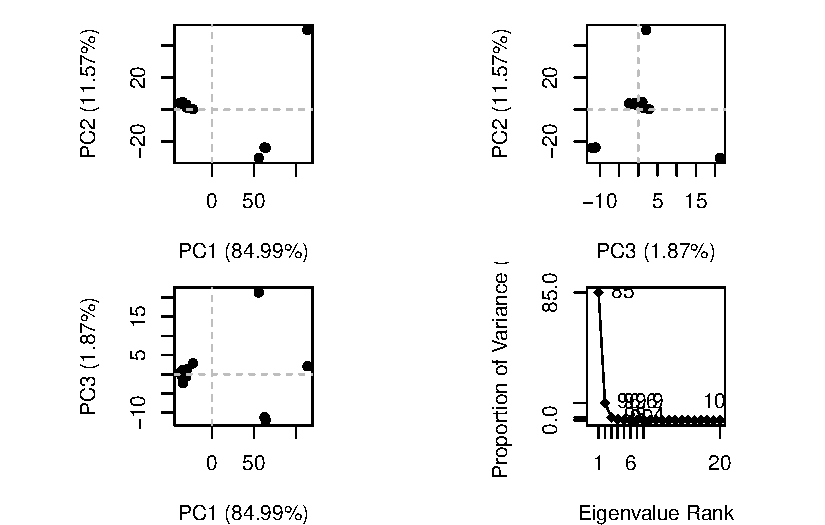
\includegraphics[keepaspectratio]{Class10_files/figure-pdf/unnamed-chunk-33-1.pdf}}

\begin{Shaded}
\begin{Highlighting}[]
\FunctionTok{plot}\NormalTok{(pc, }\DecValTok{1}\SpecialCharTok{:}\DecValTok{2}\NormalTok{)}
\end{Highlighting}
\end{Shaded}

\pandocbounded{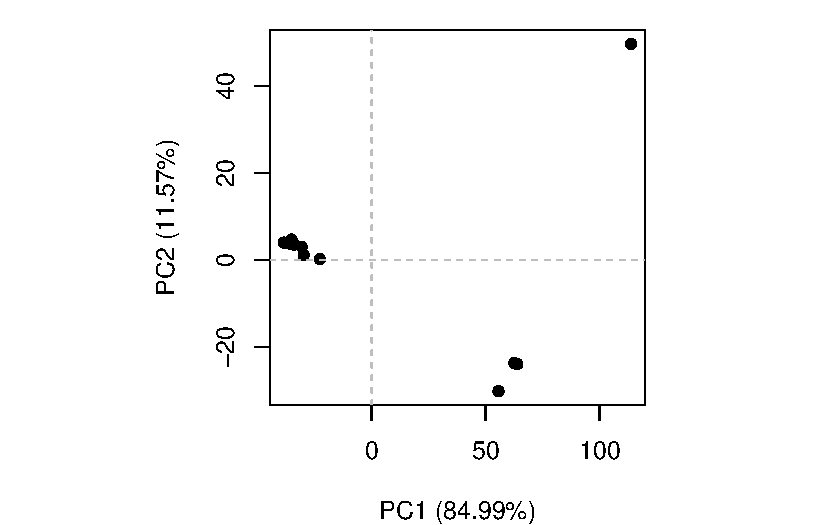
\includegraphics[keepaspectratio]{Class10_files/figure-pdf/unnamed-chunk-34-1.pdf}}

Interactive view of the PC1 captured structural differences:

\begin{Shaded}
\begin{Highlighting}[]
\CommentTok{\#view.pca(pc)}
\end{Highlighting}
\end{Shaded}

\begin{Shaded}
\begin{Highlighting}[]
\FunctionTok{mktrj}\NormalTok{(pc, }\AttributeTok{file=}\StringTok{"pca.pdb"}\NormalTok{)}
\end{Highlighting}
\end{Shaded}





\end{document}
